\documentclass[11pt, headsepline]{article}

\usepackage[top=1in, bottom=1in, left=1in, right=1in]{geometry}
\usepackage[usenames, dvipsnames]{xcolor}
\usepackage[colorlinks=true,linkcolor=blue,citecolor=Mahogany,urlcolor=blue]{hyperref}
\usepackage{booktabs, tabularx, hhline, multirow, threeparttable, longtable}
\usepackage{graphicx}
\usepackage{subcaption}
\usepackage{array}
\usepackage{amsmath}
\usepackage{float}
\usepackage{enumitem}
\usepackage{pdflscape}
\usepackage[round]{natbib}

\newcommand{\blue}[1]{\textcolor{blue}{#1}}
\newcommand{\red}[1]{\textcolor{red}{#1}}
\definecolor{darkgreen}{rgb}{0,0.5,0}
\newcommand{\nic}[1]{\noindent\textcolor{darkgreen}{[Nic: #1]}}
\newcommand{\todo}[1]{\noindent\textcolor{blue}{[To do: #1]}}

\def\labelitemi{--}

\title{Why Do Young Americans Support Redistribution?}
% Beliefs and the Emerging Generational Gap / Age Divide
% Deservingness, Zero-Sum Beliefs, and the Growing Age Divide
% /Attribution/Desert/Fairness, Incentives/Efficiency
% Beliefs, Not Circumstances
\author{Niclas Carlson\thanks{Columbia Business School, Columbia University}, Matthew E. Kahn\thanks{Department of Economics, University of Southern California}, and Romain Rancière\footnotemark[2]}

\begin{document}

\maketitle
\begin{abstract}
Young people have a stronger preference for redistribution than older people. Using a unique survey equally balanced between adults younger than and older than 30, we test several hypotheses to explain the age gap in preferences for redistribution. Difference in zero-sum beliefs and the disincentive effects of progressive taxation explain the vast majority of the gap. We confirm these results using other cross-sectional and longitudinal surveys. We find that the gap identified in our survey has been considerably widening over time and find that such widening could be explained by...
\end{abstract}

\noindent\textbf{Keywords:}

\newpage
\section{Introduction}

Headline question, historical claims and folk wisdom about link between of age and politics, important hypotheses/theories,  summary of results.

To be discussed but I would suggest a structure like this

1. Understand The Generational Gaps in Preferences for Redistribution based on several hypothesis (our survery) - the unique nature of our survey
2. Confirm with other survey the main finding (Stancheva)
3. Document the widening gap (discuss Generation vs. Period Effect)
4. Explain the widnening gap (income inequality, mobility, immigration) - this might be the part that still needs a bit of work

\subsection{Literature review}

\todo{Fill in most-important papers}

\cite{kuziemko2015elastic}:

\cite{alesina2018intergenerational}: mobility and demand for redistribution.

\cite{alesina2023immigration}: immigration and demand for redistribution.

\cite{stantcheva2021understanding}: tax understanding, efficiency/incentive beliefs, government views, and demand for redistribution.

\cite{chinoy2026zero}: zero-sum beliefs and demand for redistribution.

\cite{davidai2019politics}: liberals view economic inequality as zero-sum, conservatives view social inequality as zero-sum.

\cite{piketty1995social}:

\cite{alesina2011preferences}:

\cite{giuliano2023recessions}:

\cite{malmendier2011depression}:

\cite{benabou2006belief}:

\cite{almaas2020cutthroat}:

\cite{enke2020moral}:

older political science literature refuting self-interest hypothesis

\cite{landier2008investigating}:

\newpage
\section{A widening age gradient in redistributive preferences}

Recent surveys suggest a strong age gradient \blue{(or generational gap)} in preferences for redistribution of income/wealth.

\begin{figure}[H]
    \centering
    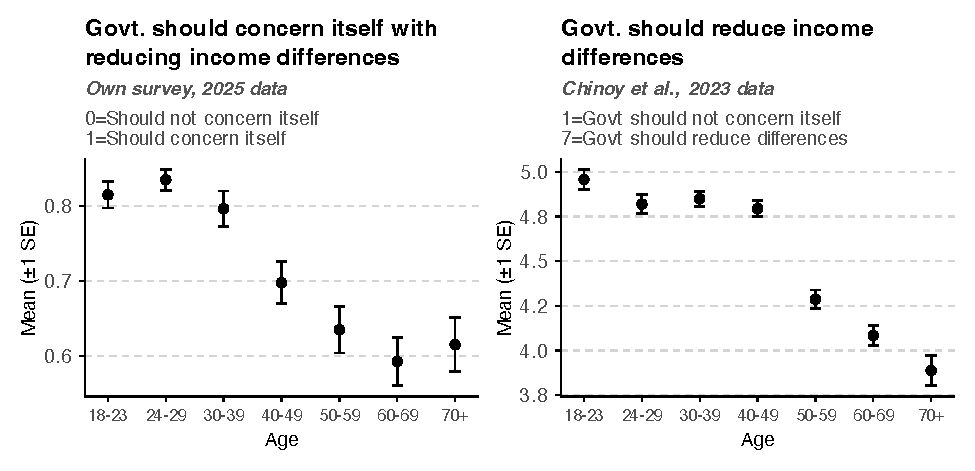
\includegraphics[width=\linewidth]{graphs/pair_shouldconcern.pdf}
\end{figure}
\todo{Need to add labels and captions to plots, add any end-notes to tables, and make some tables latex rather than pdf}

Longitudinal surveys suggest the age gradient has widened. In the 1970s/80s, any gradient is barely noticeable. 

\begin{figure}[H]
    \centering
    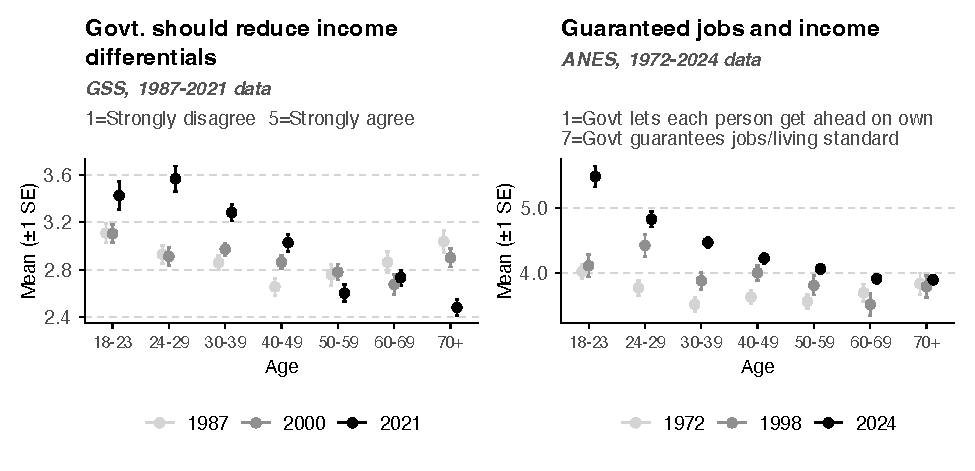
\includegraphics[width=\linewidth]{graphs/pair_headline.pdf}
\end{figure}

In our online survey data, unadjusted regressions of age on policy preferences confirm the current existence of an age divide. For the binary question ``Should the government concern itself with reducing income differences between rich and poor people?'' we use a logistic regression, and for the remainder of the section, we use simple OLS regressions. The negative age coefficient suggests that, on average, older Americans support redistribution less and younger Americans support redistribution more.

\begin{table}[H]
\caption{Single-period bivariate regressions}
\centering
\begin{threeparttable}

\begin{tabular}{lccc}
\toprule
 & shouldconcern (logit) & progressivity (OLS) & proposal (OLS) \\
\midrule
Age & -0.4572$^{***}$ & -0.1096$^{***}$ & -0.0998$^{***}$ \\
    & (0.0459) & (0.0202) & (0.0203) \\
\midrule
N & 2,415 & 2,415 & 2,415 \\
\bottomrule
\end{tabular}
\begin{tablenotes}[flushleft]
\footnotesize
\item Data: own survey, fielded 2025
\item Both age and outcome z-scored (per-SD units). All outcomes coded high =
pro-redistribution. Standard errors in parentheses.
\item $^{*}$ $p<0.1$, $^{**}$ $p<0.05$, $^{***}$ $p<0.01$.
\end{tablenotes}
\end{threeparttable}
\end{table}

Cross-checking with the most-recent waves of the GSS and ANES, plus the high-sample-size survey from \cite{chinoy2026zero} confirms the finding.
\begin{table}[H]
\caption{Single-period bivariate OLS regressions}
\centering
\begin{threeparttable}
\begin{tabular}{lccc}
\toprule
 & GSS reduce inc. diffs. & ANES guaranteed income & Chinoy et al. reduce inc. diffs. \\
\midrule
Age & -0.2573$^{***}$ & -0.2064$^{***}$ & -0.1811$^{***}$ \\
    & (0.0238) & (0.0148) & (0.0061) \\
\midrule
N & 1,710 & 4,520 & 26,730 \\
\bottomrule
\end{tabular}
\begin{tablenotes}[flushleft]
\footnotesize
\item Data: GSS fielded 2021, ANES fielded 2024, Chinoy et al. fielded 2020-23
\item Both age and outcome z-scored (per-SD units). All outcomes coded high =
pro-redistribution. Standard errors in parentheses.
\item $^{*}$ $p<0.1$, $^{**}$ $p<0.05$, $^{***}$ $p<0.01$.
\end{tablenotes}
\end{threeparttable}
\end{table}

The widening of the generational divide over time is strongly statistically significant. The negative age coefficient suggests that older Americans support redistribution less, the positive period coefficient suggests that support across the population has increased over time, and the negative coefficient on the age-period interaction suggests that in later (more recent) years, the age gradient has steepened.

\begin{table}[H]
\caption{Multi-period OLS regressions with age-period interaction}
\label{table:multi-period-regression}
\centering
\begin{threeparttable}
\begin{tabular}{lcc}
\toprule
 & GSS reduce inc. diffs. & ANES guaranteed income \\
\midrule
Age & -0.0356$^{**}$ & -0.0239$^{***}$ \\
    & (0.0153) & (0.0091) \\
Period & 0.0365$^{***}$ & 0.0428$^{***}$ \\
       & (0.0079) & (0.0027) \\
Age $\times$ Period & -0.0506$^{***}$ & -0.0278$^{***}$ \\
                    & (0.0078) & (0.0027) \\
\midrule
N & 13,071 & 45,853 \\
\bottomrule
\end{tabular}
\begin{tablenotes}[flushleft]
\footnotesize
\item Data: GSS waves 1987-2021, ANES waves 1972-2024
\item Both age and outcome z-scored (per-SD units). All outcomes coded high =
pro-redistribution. Period = decades since first wave used, kept continuous.
Standard errors in parentheses.
\item $^{*}$ $p<0.1$, $^{**}$ $p<0.05$, $^{***}$ $p<0.01$.
\item F-test of Age $\times$ Period $=0$: GSS $F=42.17$, ANES $F=106.86$.
\end{tablenotes}
\end{threeparttable}
\end{table}

\subsection{Cohort effects or age effects?}

APC is not possible to disentangle without an instrument. However, a widening of the gradient cannot come from period effects; it must come from cohort effects or time-varying age effects. Further, the graphs below can give us hints. In the following graphs, cohorts start at different means, which is partially explained by the positive period effects in table \ref{table:multi-period-regression}, but could also be due to positive cohort effects.  Preferences are somewhat stable over time, suggesting cohort effects, but there is some downward trending over the life-cycle, suggesting some age effects (especially if period effects are trending the opposite direction). Later sections will test whether mechanisms seem more consistent with the age/lifecycle hypothesis versus the cohort/imprinting hypothesis. 

\begin{figure}[H]
    \centering
    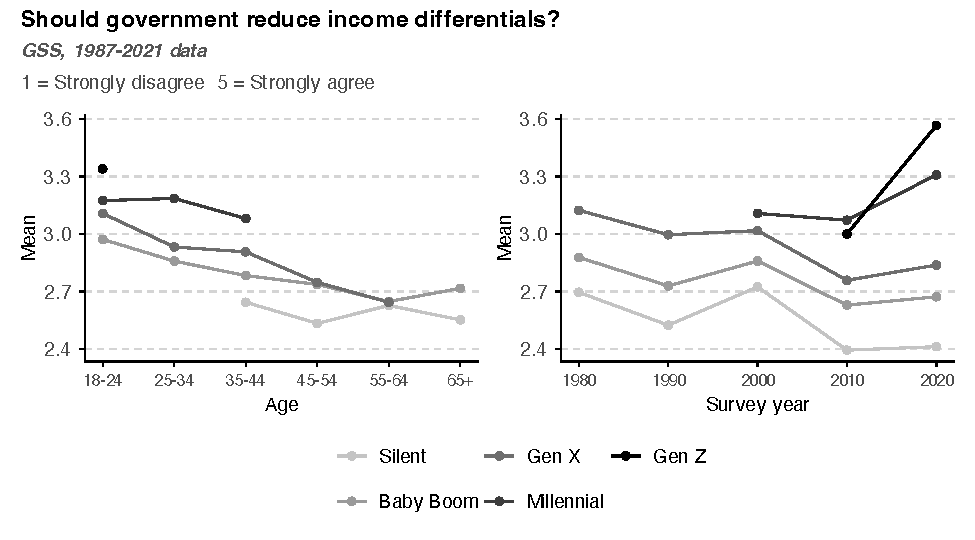
\includegraphics[width=\linewidth]{graphs/pair_apc_GSS_GOVEQINC.pdf}
\end{figure}
\begin{figure}[H]
    \centering
    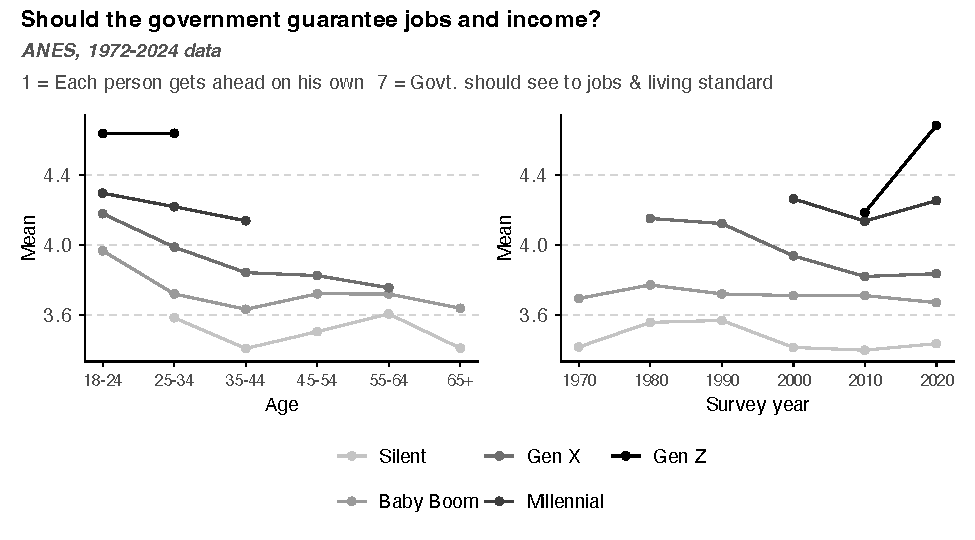
\includegraphics[width=\linewidth]{graphs/pair_apc_ANES_VCF0809.pdf}
\end{figure}

Plotting age versus predicted mean preferences with birth-decade (cohort) versus with survey-year (period) fixed effects suggests that cohort effects drive a large portion of the age gradient while, as we would expect, period effects do not drive the age gradient; after controlling for birth-decade fixed effects, the slope of age versus demand for redistribution shrinks, while controlling for survey-year fixed effects does not alter the age-preference slope. 

\begin{figure}[H]
\centering
\begin{subfigure}{0.48\textwidth}
    \centering
    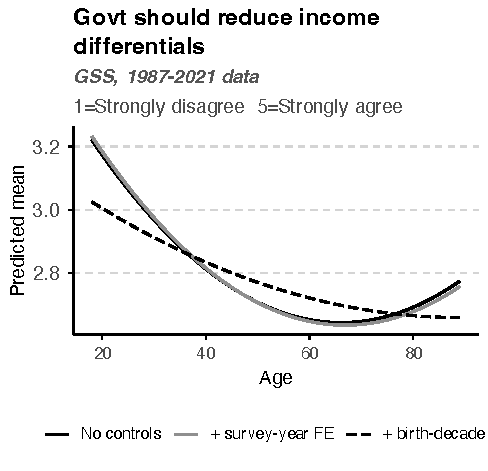
\includegraphics[width=\textwidth]{graphs/fe_GSS_GOVEQINC.pdf}
\end{subfigure}
\hfill
\begin{subfigure}{0.48\textwidth}
    \centering
    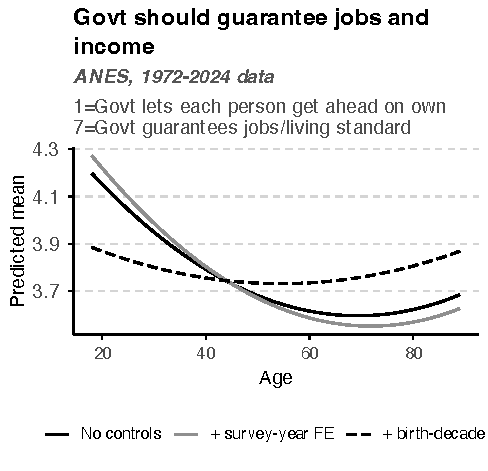
\includegraphics[width=\textwidth]{graphs/fe_ANES_VCF0809.pdf}
\end{subfigure}
% \caption{Overall figure title}
% \label{fig:overall}
\end{figure}



\newpage
\section{The life-cycle hypothesis: rationality under financial uncertainty}
% financial position and risks

\subsection{Survey design}

\todo{Describe wave 1 questionnaire, Prolific bot process, and summary statistics.}

\subsection{Empirical tests: weak evidence}

\todo{Insert tests/falsification.}

Three main hypotheses: (i) current income and financial strain, which is the level of financial position, (ii) perceived income/career/other financial risk (climate, housing prices, etc.), which is the variance of financial position, and (iii) expected trajectory and consumption smoothing, which is the path of financial position. Current unemployment, financial satisfaction, savings levels, and income belong to (i). The variance and lower bound of expected income and perceived exposure to climate/AI/housing risk belong to (ii). Expected growth or stagnation in income, the upper bound of expected income, myopia and time-discounting belong in (iii). 

The most simple way to test (i)–(iii) would be head-to-head against other variables. We could construct variables that proxy for each channel, including interactions such as myopia x expected income growth or downside income risk x perceived mobility, then compare the R-squared attributed to each channel in a Shapley decomposition. We will probably find that beliefs matter much more. 

So far, we find statistically significant but quantitatively small evidence that redistribution functions as insurance for longer-term risks which young people are more exposed to such as income/career uncertainty, housing, climate, and AI; weak evidence that redistribution functions as relief from present financial stress, which may be higher among young people; weak evidence that young people, who are often poorer earlier in their careers, favor redistribution due to myopia or time-discounting; and weak evidence that young people support redistribution because of misperceived future income needs or lack of experience with taxation.

\todo{Reference theory/empirics from the literature for each of the hypotheses above.}

\nic{Values/personality traits such as generosity, materialism, and universalism/individualism could plausibly change over the life cycle, but we find them to weakly predict preferences for redistribution.}

\newpage
\section{The cohort-imprinting hypothesis: beliefs about the economic game}

\nic{Could be a lifecycle aspect to some of these beliefs, so the title may be claiming too much.}

\subsection{Mechanism clusters and sample coverage}

The following tables describe the definitions of the variable clusters used in later sections and the number of questions fielded in each survey that fall within a cluster (our own, longitudinal, or recently-published data).

\begingroup\footnotesize\renewcommand{\arraystretch}{0.92}
\begin{longtable}{@{}p{2.2in} p{3.7in}@{}}
\caption{What each candidate cluster measures}\label{tab:clusters_glossary}\\
\toprule Cluster & Description \\ \midrule\endfirsthead
\toprule Cluster & Description \\ \midrule\endhead
\multicolumn{2}{@{}l}{\bfseries demographics}\\[2pt]
\quad age & Age in years \\
\quad citizenship & Respondent and parents' birthplace and immigrant status \\
\quad gender & Gender \\
\quad marital status & Married cohabiting or single \\
\quad race & Race and ethnicity \\
\addlinespace[4pt]
\multicolumn{2}{@{}l}{\bfseries position}\\[2pt]
\quad ai/tech risk & Exposure to job loss from AI and whether technology helps \\
\quad education & Highest level of education completed \\
\quad employment & Employment status and hours \\
\quad family income / background & Income, education and occupation of the respondent's parents and grandparents \\
\quad financial stress/risk & Savings buffer income stability and financial satisfaction \\
\quad health insurance & Insurance coverage and the risk of losing it \\
\quad homeownership & Owning versus renting now and in childhood \\
\quad income & Household income now expected and needed to live comfortably \\
\quad location density & Urban suburban or rural residence \\
\quad social class & Subjective social class and the respondent's own occupation and standing \\
\quad unemployment risk & Job security and expected ease of re-employment \\
\addlinespace[4pt]
\multicolumn{2}{@{}l}{\bfseries beliefs}\\[2pt]
\quad aggregate incentives / inequality positive-sum & Whether large pay gaps are needed to motivate effort and grow the pie \\
\quad class conflict & Perceived conflict between rich and poor \\
\quad deservingness of poor & Whether poverty reflects lack of effort or circumstance \\
\quad discrimination & Whether minorities are seen as disadvantaged by discrimination and blocked opportunity, or by ability and effort \\
\quad equality/dei zero-sum & Whether gains for women and minorities come at others' expense \\
\quad experienced mobility & Whether the respondent's own effort and schooling have paid off, and how they compare with their parents \\
\quad factual knowledge / misperceptions & Accuracy about verifiable economic facts: tax rates, who pays them, and how much the top 1 percent gained \\
\quad government integrity / capability & Whether government is trustworthy, run for everyone, and able to reduce unequal opportunity \\
\quad immigration & Perceived effect of immigrants and what makes someone truly American \\
\quad individual incentives & Whether extra pay induces effort skill and schooling \\
\quad individual incentives / tax elasticity & Whether higher taxes would make high earners and the middle class work less \\
\quad inequality perception & Perceived change in the top 1 percent income share \\
\quad other zero-sum & Zero-sum thinking about international trade \\
\quad perceived mobility / opportunity & Perceived chance a poor child rises and whether mobility is falling \\
\quad policy incidence & Who is believed to gain or lose when high earners are taxed \\
\quad social trust & Whether most people can be trusted or would take advantage \\
\quad wealth from advantages & Whether getting ahead requires connections family and luck \\
\quad wealth from effort/merit & Whether hard work rather than luck explains who succeeds \\
\quad wealth zero-sum & Whether the rich gain at others' expense rather than creating value \\
\addlinespace[4pt]
\multicolumn{2}{@{}l}{\bfseries worldview/values}\\[2pt]
\quad climate/environment concern & Climate risk exposure and environmental engagement \\
\quad distributive principle / desert & What pay ought to depend on and whether own pay is just \\
\quad generosity / universalism & How much is given to others and how wide the circle of concern is, from close ties to strangers \\
\quad materialism / ideal lifestyle & What the respondent values in a job and in life \\
\quad patience & Time preference over money and long-term goals \\
\quad religiosity & Importance of religion and frequency of attendance \\
\addlinespace[3pt]\midrule\addlinespace[3pt]
\multicolumn{2}{@{}l}{\bfseries redistributive preferences}\\[2pt]
\quad policy helping poor & Support for spending, services and guarantees aimed at low-income Americans \\
\quad policy redistributive & Whether government should reduce income differences -- the paper's main outcomes \\
\quad policy tax & Preferred tax rates and whether current taxes are fair \\
\addlinespace[4pt]
\multicolumn{2}{@{}l}{\bfseries other preferences}\\[2pt]
\quad fairness of the current distribution & Whether the existing distribution and economic system are fair or a serious problem \\
\quad government scope & How much government should do overall, beyond redistribution specifically \\
\quad immigration policy & Whether immigration should be increased or restricted \\
\quad preferential hiring & Support for preferential hiring of women or minorities \\
\quad stated reasons for own view change & Respondent's own account of why their redistribution views shifted \\
\quad tax incidence / trickle-down & Who is claimed to gain when taxes on high earners are cut \\
\bottomrule
\end{longtable}\endgroup

% \cite{stantcheva2021understanding} claims to rule out efficiency hypothesis, but only ask whether taxes on the rich make the rich work less (not whether lower income people would work less hard to become rich). 

% Further, she claims that government confidence is more important, when the variable used is tautological, asking the respondent whether ``the government should do more to solve our country's problems.'' In fact, removing that question and other tautological questions such as ``inequality is a serious problem'' and ``wealthy people are entitled to keep their money,'' the \textit{most} important variable in a Shapley decomposition is ``raising income tax on high earners would hurt/help the economy.'' The divide between what is a (relatively more primitive) belief and what is a preference is not explicitly discussed in this literature, and the failure to draw a line could lead to inconsistent results.

We will find that although we consider a diverse range of beliefs, viewpoints, values, demographics and personal situations, a very small subset of variables---beliefs about the economic game---predict preferences for redistribution and explain the age gradient. No existing survey covers every major belief cluster (including our own, although it is broader than most).

\nic{A Prolific wave 2 opportunity: disentangling related-but-distinct beliefs: What are the primitive beliefs driving things? Is it economic zero-sum, social zero-sum, causal attribution/deservingness, opportunity, or incentive effects? Which of these are distinct/orthogonal belief clusters? When we distinguish between them, which emerges as most important? }


\begin{landscape}

\begingroup\footnotesize\setlength{\tabcolsep}{4pt}\renewcommand{\arraystretch}{0.92}
\begin{longtable}{@{}l p{2.6in} ccc cccc@{}}
\caption{Survey coverage}\label{tab:clusters_wide}\\
\toprule
Group & Cluster & GSS & ANES & WVS (US) & Own & Chinoy & Stant. & Alesina \\
\midrule\endfirsthead
\toprule
Group & Cluster & GSS & ANES & WVS (US) & Own & Chinoy & Stant. & Alesina \\
\midrule\endhead
demographics & age & 1~(1972-2024) & 1~(1952-2024) & 1~(1995-2017) & 1 & 1 & 1 & 1 \\
 & citizenship & 1~(1977-2024) & \textcolor[gray]{0.62}{--} & 3~(2006-2017) & 2 & 1 & \textcolor[gray]{0.62}{--} & 2 \\
 & gender & 1~(1972-2024) & 1~(1948-2024) & 1~(1995-2017) & 3 & 1 & 1 & 1 \\
 & marital status & \textcolor[gray]{0.62}{--} & 1~(1952-2024) & 1~(1995-2017) & 3 & 1 & 1 & 1 \\
 & race & \textcolor[gray]{0.62}{--} & 1~(1948-2024) & 1~(1995-2017) & 5 & 1 & 1 & \textcolor[gray]{0.62}{--} \\
\addlinespace[2pt]
position & ai/tech risk & \textcolor[gray]{0.62}{--} & \textcolor[gray]{0.62}{--} & 3~(2006-2017) & 1 & \textcolor[gray]{0.62}{--} & \textcolor[gray]{0.62}{--} & \textcolor[gray]{0.62}{--} \\
 & education & \textcolor[gray]{0.62}{--} & 1~(1948-2024) & 1~(1995-2017) & 1 & 1 & 1 & 1 \\
 & employment & 1~(1972-2024) & 1~(1952-2024) & 1~(1995-2017) & 7 & 1 & 1 & 1 \\
 & family income / background & 3~(1972-2024) & 1~(1952-1996) & 3~(2017) & 5 & 6 & \textcolor[gray]{0.62}{--} & 3 \\
 & financial stress/risk & 3~(1972-2024) & 2~(1956-2024) & 2~(1995-2017) & 2 & \textcolor[gray]{0.62}{--} & \textcolor[gray]{0.62}{--} & \textcolor[gray]{0.62}{--} \\
 & health insurance & 1~(1991-2004) & 1~(1992-2024) & \textcolor[gray]{0.62}{--} & 1 & \textcolor[gray]{0.62}{--} & \textcolor[gray]{0.62}{--} & \textcolor[gray]{0.62}{--} \\
 & homeownership & 2~(1985-2024) & 1~(1952-2024) & \textcolor[gray]{0.62}{--} & 1 & \textcolor[gray]{0.62}{--} & \textcolor[gray]{0.62}{--} & \textcolor[gray]{0.62}{--} \\
 & income & 3~(1972-2024) & 4~(1948-2024) & 1~(1995-2017) & 5 & 3 & 1 & 1 \\
 & location density & 3~(1972-2024) & 1~(1952-2000) & 2~(1995-2017) & 2 & 1 & \textcolor[gray]{0.62}{--} & \textcolor[gray]{0.62}{--} \\
 & social class & 3~(1972-2024) & 3~(1952-2016) & 1~(1995-2017) & 1 & \textcolor[gray]{0.62}{--} & 1 & 1 \\
 & unemployment risk & 3~(1973-2024) & 5~(1984-2024) & 1~(1995-1999) & 2 & \textcolor[gray]{0.62}{--} & \textcolor[gray]{0.62}{--} & \textcolor[gray]{0.62}{--} \\
\addlinespace[2pt]
beliefs & aggregate incentives / inequality positive-sum & 3~(1987-2021) & \textcolor[gray]{0.62}{--} & 1~(1995-2017) & 1 & \textcolor[gray]{0.62}{--} & 3 & \textcolor[gray]{0.62}{--} \\
 & class conflict & 2~(1987-2021) & \textcolor[gray]{0.62}{--} & \textcolor[gray]{0.62}{--} & \textcolor[gray]{0.62}{--} & \textcolor[gray]{0.62}{--} & \textcolor[gray]{0.62}{--} & \textcolor[gray]{0.62}{--} \\
 & deservingness of poor & 1~(2018) & \textcolor[gray]{0.62}{--} & 1~(1999-2017) & \textcolor[gray]{0.62}{--} & \textcolor[gray]{0.62}{--} & \textcolor[gray]{0.62}{--} & 1 \\
 & discrimination & 11~(1990-2024) & 2~(1986-2024) & \textcolor[gray]{0.62}{--} & \textcolor[gray]{0.62}{--} & 3 & \textcolor[gray]{0.62}{--} & \textcolor[gray]{0.62}{--} \\
 & equality/dei zero-sum & 1 & 1~(1984-2012) & \textcolor[gray]{0.62}{--} & 2 & 2 & \textcolor[gray]{0.62}{--} & \textcolor[gray]{0.62}{--} \\
 & experienced mobility & 3~(1989-2024) & \textcolor[gray]{0.62}{--} & \textcolor[gray]{0.62}{--} & 3 & 1 & \textcolor[gray]{0.62}{--} & 2 \\
 & factual knowledge / misperceptions & \textcolor[gray]{0.62}{--} & \textcolor[gray]{0.62}{--} & \textcolor[gray]{0.62}{--} & \textcolor[gray]{0.62}{--} & 1 & 5 & \textcolor[gray]{0.62}{--} \\
 & government integrity / capability & \textcolor[gray]{0.62}{--} & 3~(1958-2024) & 2~(1995-2017) & \textcolor[gray]{0.62}{--} & 1 & 1 & 2 \\
 & immigration & 4~(1996-2024) & 1~(2004-2024) & 2~(1995-2017) & \textcolor[gray]{0.62}{--} & 1 & \textcolor[gray]{0.62}{--} & \textcolor[gray]{0.62}{--} \\
 & individual incentives & 3~(1987-2000) & \textcolor[gray]{0.62}{--} & \textcolor[gray]{0.62}{--} & \textcolor[gray]{0.62}{--} & \textcolor[gray]{0.62}{--} & \textcolor[gray]{0.62}{--} & \textcolor[gray]{0.62}{--} \\
 & individual incentives / tax elasticity & \textcolor[gray]{0.62}{--} & \textcolor[gray]{0.62}{--} & \textcolor[gray]{0.62}{--} & 1 & \textcolor[gray]{0.62}{--} & 12 & \textcolor[gray]{0.62}{--} \\
 & inequality perception & \textcolor[gray]{0.62}{--} & 2~(2004-2020) & \textcolor[gray]{0.62}{--} & \textcolor[gray]{0.62}{--} & \textcolor[gray]{0.62}{--} & 2 & \textcolor[gray]{0.62}{--} \\
 & other zero-sum & \textcolor[gray]{0.62}{--} & \textcolor[gray]{0.62}{--} & \textcolor[gray]{0.62}{--} & \textcolor[gray]{0.62}{--} & 1 & \textcolor[gray]{0.62}{--} & \textcolor[gray]{0.62}{--} \\
 & perceived mobility / opportunity & \textcolor[gray]{0.62}{--} & \textcolor[gray]{0.62}{--} & \textcolor[gray]{0.62}{--} & 3 & 12 & \textcolor[gray]{0.62}{--} & 5 \\
 & policy incidence & 1~(1987-2021) & \textcolor[gray]{0.62}{--} & \textcolor[gray]{0.62}{--} & \textcolor[gray]{0.62}{--} & \textcolor[gray]{0.62}{--} & 10 & \textcolor[gray]{0.62}{--} \\
 & social trust & 2~(1972-2024) & 3~(1964-2020) & 3~(1995-2017) & \textcolor[gray]{0.62}{--} & 1 & \textcolor[gray]{0.62}{--} & \textcolor[gray]{0.62}{--} \\
 & wealth from advantages & 11~(1987-2021) & \textcolor[gray]{0.62}{--} & \textcolor[gray]{0.62}{--} & \textcolor[gray]{0.62}{--} & \textcolor[gray]{0.62}{--} & \textcolor[gray]{0.62}{--} & \textcolor[gray]{0.62}{--} \\
 & wealth from effort/merit & 7~(1973-2024) & \textcolor[gray]{0.62}{--} & 2~(1995-2017) & \textcolor[gray]{0.62}{--} & \textcolor[gray]{0.62}{--} & 1 & 1 \\
 & wealth zero-sum & 4~(1978-2024) & \textcolor[gray]{0.62}{--} & 1~(1995-2011) & 2 & 2 & \textcolor[gray]{0.62}{--} & \textcolor[gray]{0.62}{--} \\
\addlinespace[2pt]
worldview/values & climate/environment concern & 1~(2021) & 2~(1984-2024) & 4~(1995-2017) & 1 & \textcolor[gray]{0.62}{--} & \textcolor[gray]{0.62}{--} & \textcolor[gray]{0.62}{--} \\
 & distributive principle / desert & 8~(1990-2021) & \textcolor[gray]{0.62}{--} & \textcolor[gray]{0.62}{--} & \textcolor[gray]{0.62}{--} & \textcolor[gray]{0.62}{--} & 1 & \textcolor[gray]{0.62}{--} \\
 & generosity / universalism & \textcolor[gray]{0.62}{--} & 1~(1992-2024) & 3~(1995-2017) & 2 & 4 & \textcolor[gray]{0.62}{--} & \textcolor[gray]{0.62}{--} \\
 & materialism / ideal lifestyle & 5~(1989-2024) & \textcolor[gray]{0.62}{--} & 8~(1995-2017) & 7 & \textcolor[gray]{0.62}{--} & \textcolor[gray]{0.62}{--} & \textcolor[gray]{0.62}{--} \\
 & patience & \textcolor[gray]{0.62}{--} & \textcolor[gray]{0.62}{--} & 1~(1995-2017) & 7 & \textcolor[gray]{0.62}{--} & \textcolor[gray]{0.62}{--} & \textcolor[gray]{0.62}{--} \\
 & religiosity & 3~(1972-2024) & 2~(1970-2024) & 2~(1995-2017) & \textcolor[gray]{0.62}{--} & 1 & \textcolor[gray]{0.62}{--} & \textcolor[gray]{0.62}{--} \\
\addlinespace[3pt]\midrule\addlinespace[3pt]
redistributive preferences & policy helping poor & 3~(1975-2024) & 8~(1956-2024) & 2~(1995-2017) & 3 & 2 & 5 & \textcolor[gray]{0.62}{--} \\
 & policy redistributive & 2~(1978-2024) & \textcolor[gray]{0.62}{--} & 1~(1995-2017) & 1 & 1 & 3 & \textcolor[gray]{0.62}{--} \\
 & policy tax & 3~(1987-2021) & \textcolor[gray]{0.62}{--} & \textcolor[gray]{0.62}{--} & 4 & 2 & 5 & 5 \\
\addlinespace[2pt]
other preferences & fairness of the current distribution & 1~(1987-2021) & \textcolor[gray]{0.62}{--} & 1~(2006-2017) & \textcolor[gray]{0.62}{--} & 1 & 4 & 2 \\
 & government scope & 1 & 2~(1984-2024) & \textcolor[gray]{0.62}{--} & \textcolor[gray]{0.62}{--} & 1 & 2 & 2 \\
 & immigration policy & 1~(1996-2014) & 1~(1992-2024) & 2~(1995-2017) & \textcolor[gray]{0.62}{--} & 1 & \textcolor[gray]{0.62}{--} & \textcolor[gray]{0.62}{--} \\
 & preferential hiring & 1~(1996-2024) & 1~(1986-2024) & \textcolor[gray]{0.62}{--} & \textcolor[gray]{0.62}{--} & 1 & \textcolor[gray]{0.62}{--} & \textcolor[gray]{0.62}{--} \\
 & stated reasons for own view change & \textcolor[gray]{0.62}{--} & \textcolor[gray]{0.62}{--} & \textcolor[gray]{0.62}{--} & 9 & \textcolor[gray]{0.62}{--} & \textcolor[gray]{0.62}{--} & \textcolor[gray]{0.62}{--} \\
 & tax incidence / trickle-down & \textcolor[gray]{0.62}{--} & \textcolor[gray]{0.62}{--} & \textcolor[gray]{0.62}{--} & \textcolor[gray]{0.62}{--} & \textcolor[gray]{0.62}{--} & 1 & 1 \\
\bottomrule
\end{longtable}
\vspace{-6pt}\noindent{\scriptsize Question inventory for the Section 4.1 decomposition. Cells give the number of questions the survey \emph{asks} in that cluster; \textcolor[gray]{0.62}{--} marks a cluster the survey does not measure at all. Above the rule are the 372 candidate items, of which 356 enter our battery; the rest are catalogued for coverage but stay out of the models. \textbf{Below the rule} are the 86 \emph{preference} items -- the outcomes themselves and normative \emph{should government} questions -- shown for coverage but excluded from the decomposition by construction, since they restate what we are trying to explain. Ideology and civic participation are omitted entirely. GSS counts are our 107-variable extract plus known relevant items from the full GSS (flagged in the catalog), which holds thousands more -- a curated lower bound, not an exhaustive inventory. WVS is US respondents only. For GSS, ANES and WVS (US) the parenthetical is the span of years those questions were actually fielded, which varies widely within a survey; the cross-sections were each fielded once: Own survey, 2025; Chinoy et al., 2020-23; Stantcheva, 2019; Alesina et al., 2016. \ Cluster wording is ours.}\par
\endgroup
    
\end{landscape}

\subsection{Shapley decomposition: most-important predictors of preferences}

\todo{Insert classes of variables collected/used in the longitudinal surveys. Chose candidate correlates representing every hypothesis I could think of from the literature.}

A Shapely decomposition splits a regression's R-squared across predictors. To handle correlated predictors fairly, the method averages each predictor's marginal contribution over all possible orderings of entry. Shares are non-negative and sum to the full model's R-squared, so each number is interpreted as that variable's percentage of explained variance. In the ``by cluster'' tables, we simply sum the percentage explained by each variable in the cluster.

In the tables below, Shapley decompositions for a range of surveys suggest that beliefs about the zero-sumness of wealth and social/racial equality are the most important predictors of redistributive preferences, followed by beliefs about deservingness/attribution, aggregate efficiency, and opportunity/mobility. 

Our online survey suggests the importance of beliefs relating to aggregate efficiency, the zero-sumness of wealth, and the zero-sumness of DEI initiatives.

\begin{figure}[H]
    \centering
    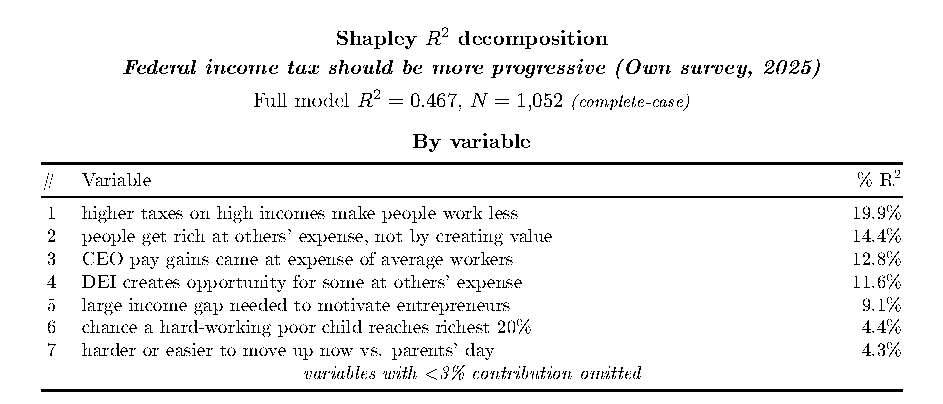
\includegraphics[width=\linewidth]{tables/07_prolific_progressivity_variable.pdf}
\end{figure}
\begin{figure}[H]
    \centering
    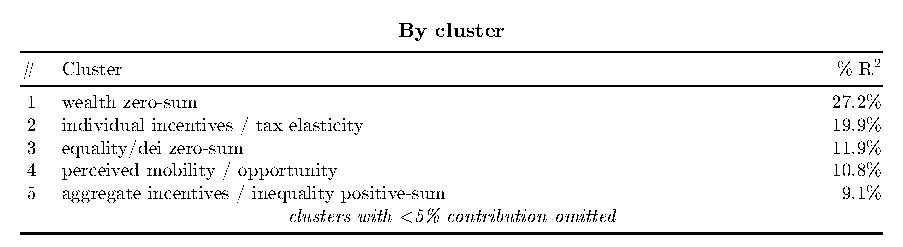
\includegraphics[width=\linewidth]{tables/07_prolific_progressivity_cluster.pdf}
\end{figure}

\begin{figure}[H]
    \centering
    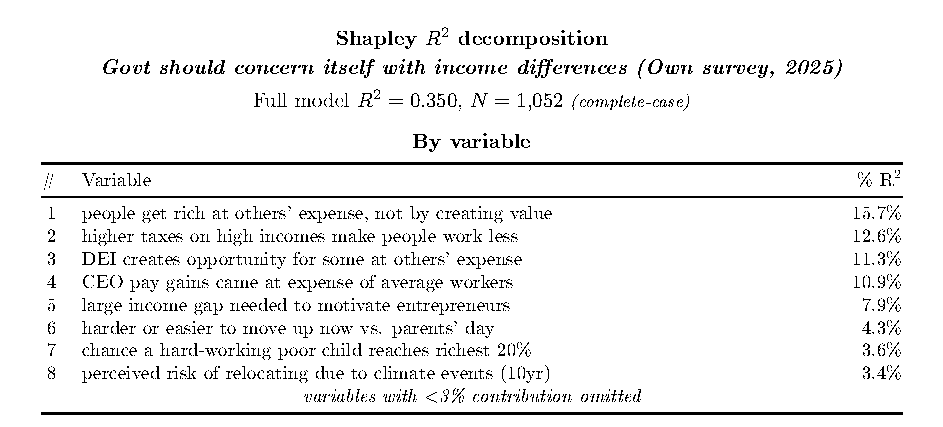
\includegraphics[width=\linewidth]{tables/09_prolific_shouldconcern_variable.pdf}
\end{figure}
\begin{figure}[H]
    \centering
    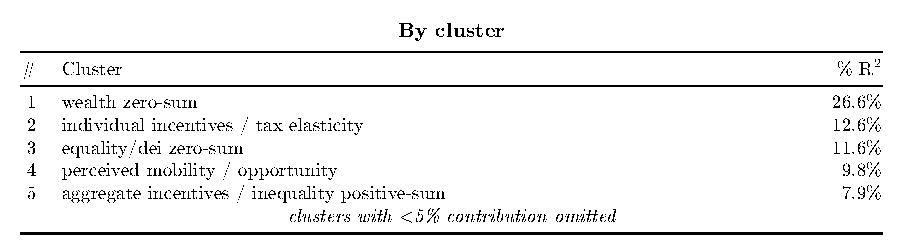
\includegraphics[width=\linewidth]{tables/09_prolific_shouldconcern_cluster.pdf}
\end{figure}

Data from \cite{chinoy2026zero} suggests the importance of discrimination, zero-sum ethnicity, zero-sum wealth, and to a lesser extent, mobility/opportunity.

\begin{figure}[H]
    \centering
    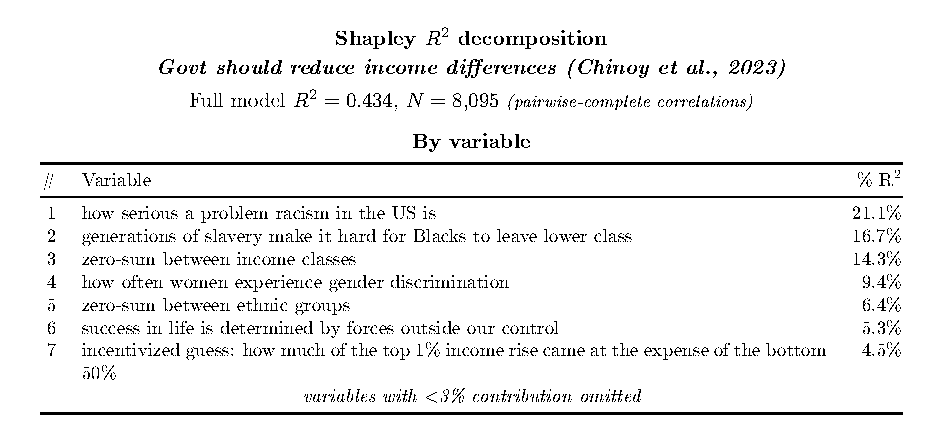
\includegraphics[width=\linewidth]{tables/10_chinoy_gov_outcome_variable.pdf}
\end{figure}
\begin{figure}[H]
    \centering
    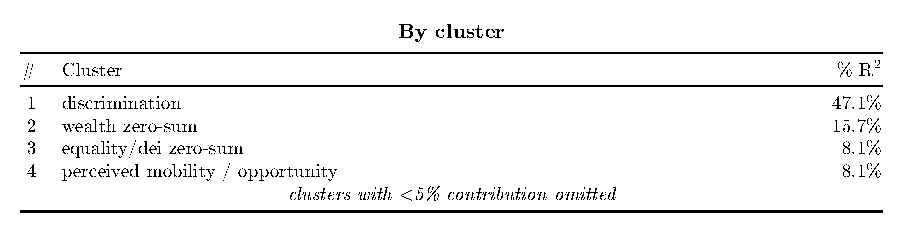
\includegraphics[width=\linewidth]{tables/10_chinoy_gov_outcome_cluster.pdf}
\end{figure}

While \cite{stantcheva2021understanding} originally found that views about the government are more important than efficiency concerns, when we remove questions about what the government should do (this is a subjective matter of drawing a line between beliefs and preferences), a different picture emerges; aggregate efficiency, policy incidence, and attribution/deservingness seem most important, though R-squared in the model is low.

\begin{figure}[H]
    \centering
    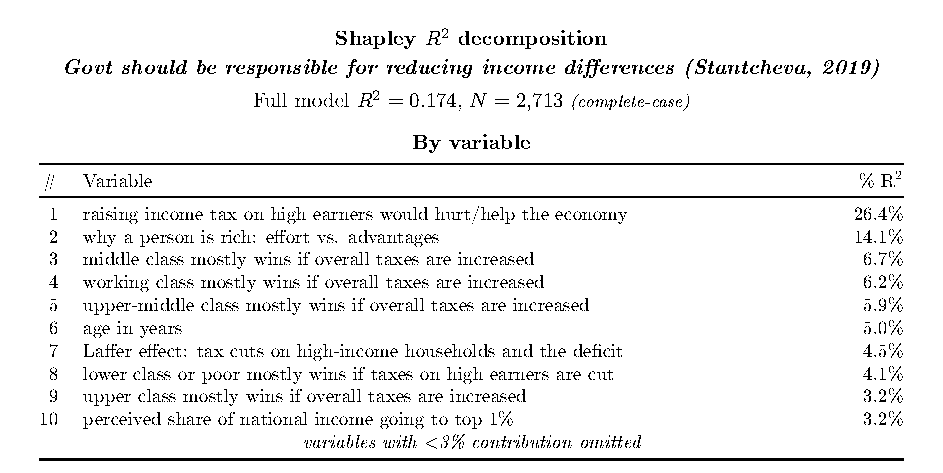
\includegraphics[width=\linewidth]{tables/12_stantcheva_dummy_g10006_1_variable.pdf}
\end{figure}
\begin{figure}[H]
    \centering
    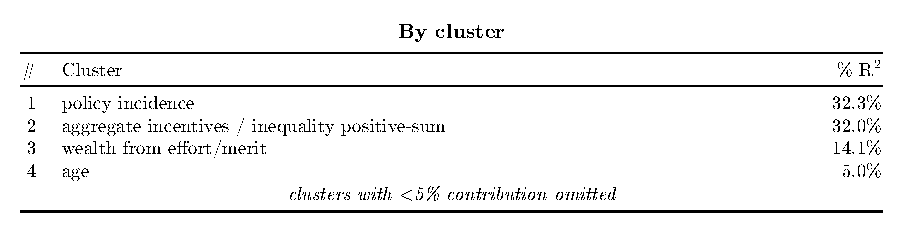
\includegraphics[width=\linewidth]{tables/12_stantcheva_dummy_g10006_1_cluster.pdf}
\end{figure}

ANES features few questions about relevant economic beliefs, and WVS has good questions but poor coverage for the same respondents in the same year, so GSS has the least-deficient longitudinal data for a Shapely decomposition. In the GSS data, zero-sum wealth, perceived class conflict, and attribution/deservingness are the most-predictive clusters.

\begin{figure}[H]
    \centering
    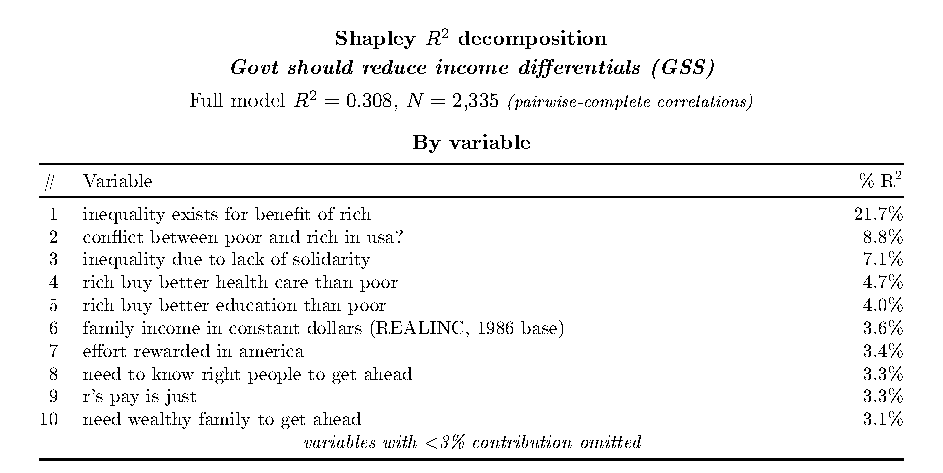
\includegraphics[width=\linewidth]{tables/02_gss_goveqinc_variable.pdf}
\end{figure}
\begin{figure}[H]
    \centering
    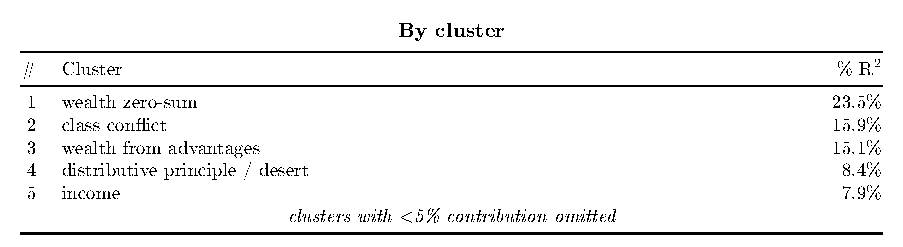
\includegraphics[width=\linewidth]{tables/02_gss_goveqinc_cluster.pdf}
\end{figure}


\newpage
\section{Can divergence in beliefs explain divergence in preferences?}

\subsection{Age gradients in beliefs: suggestive graphs}

Our online survey and \cite{chinoy2026zero} find strong age gradients in zero-sum wealth beliefs: young people on average are more likely to believe that people become wealthy by taking from others.

\begin{figure}[H]
    \centering
    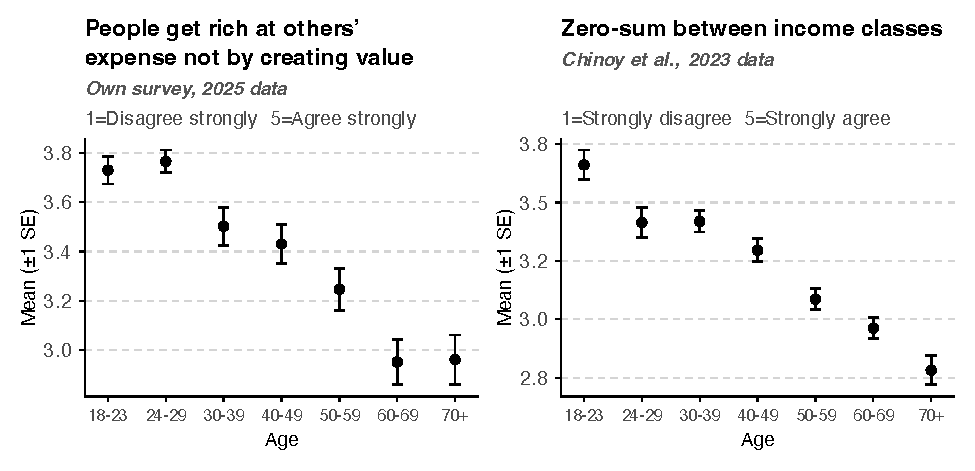
\includegraphics[width=\linewidth]{graphs/pair_zerosum_wealth.pdf}
\end{figure}

The WVS also displays prominent age gradients in a question gauging beliefs about mobility and attribution of success. We will find this theme (deservingness/opportunity) to be important in the Gelbach decomposition for the GSS.

\begin{figure}[H]
    \centering
    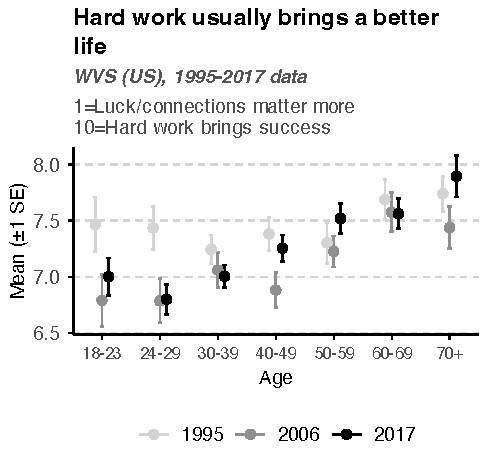
\includegraphics[width=.5\linewidth]{graphs/WVS_E040_evl.pdf}
\end{figure}

While our online survey finds that young people see DEI as less zero-sum, \cite{chinoy2026zero} finds that young people see ethnic group gains as \textit{more} zero-sum; young people are more likely to agree with the statement ``If one ethnic group becomes richer, this generally comes at the expense of other groups in the country.'' I think the latter result could be due to framing: getting ``richer'' implies the majority group, so respondents are primed to think about rich whites getting richer, not poor non-whites getting richer. 

\begin{figure}[H]
    \centering
    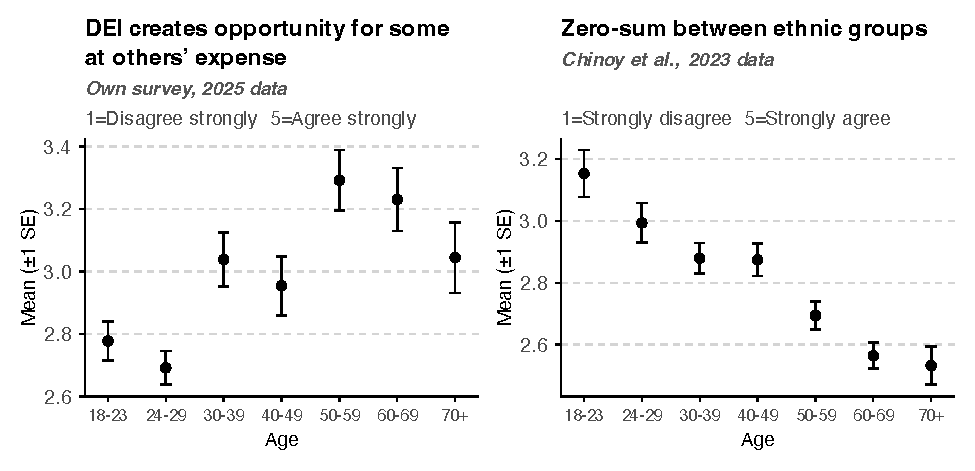
\includegraphics[width=\linewidth]{graphs/pair_zerosum_social.pdf}
\end{figure}

Backing up the point that framing could be the issue, young people are less likely to think that non-citizens' income is zero-sum and more likely to think racism is a problem (admittedly, not the exact same question, but related).

\begin{figure}[H]
    \centering
    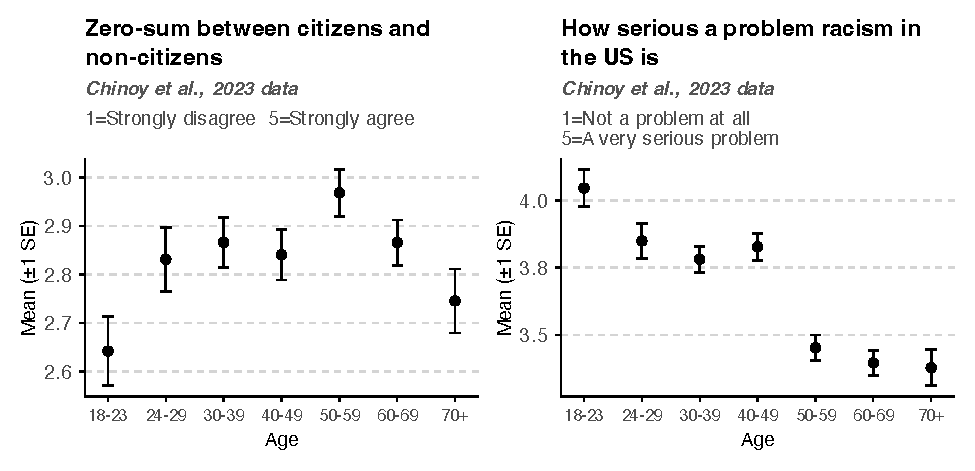
\includegraphics[width=\linewidth]{graphs/pair_framing_check.pdf}
\end{figure}





Our only long-running zero-sum wealth question, from the WVS, is inconclusive about whether the gradient has widened over time. However, the GSS shows that young people are much more likely nowadays to believe that rich people benefit from structural advantages.

\begin{figure}[H]
    \centering
    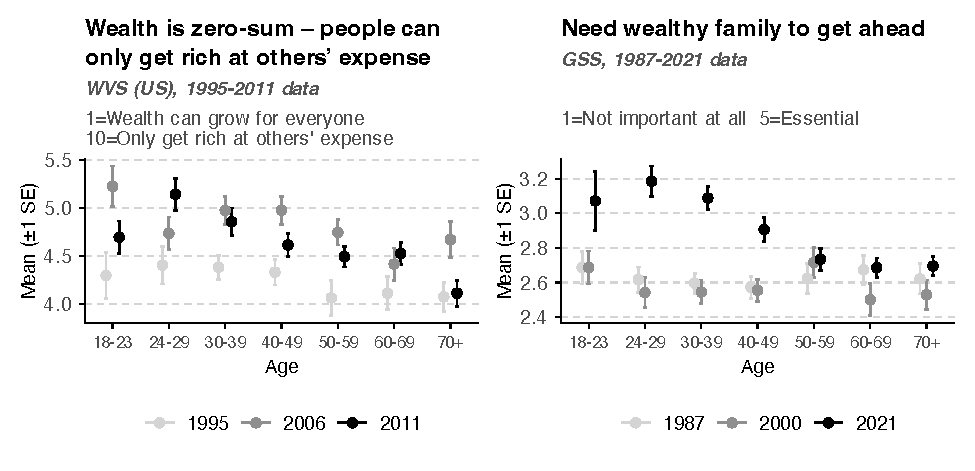
\includegraphics[width=\linewidth]{graphs/pair_zerosum_longrun.pdf}
\end{figure}

Though there is no long-running zero-sum race/social equality question, the ANES suggests that the age gradient in support for affirmative action is widening. The rise in the share of non-whites in younger cohorts could be part of the explanation.

\begin{figure}[H]
    \centering
    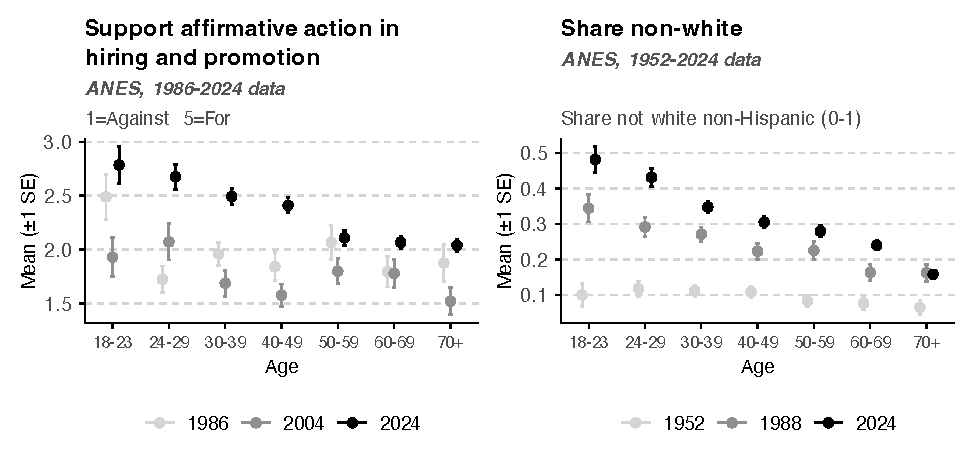
\includegraphics[width=\linewidth]{graphs/pair_race_longrun.pdf}
\end{figure}

There also seems to be an evolving gradient in perceived economic situation: younger people nowadays are less likely to feel that their financial situation has improved or that they are in a high income class.

\begin{figure}[H]
    \centering
    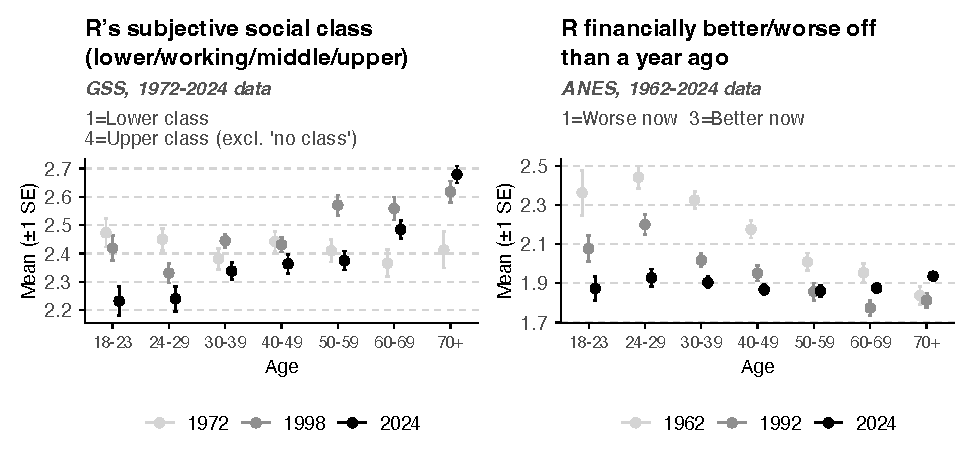
\includegraphics[width=\linewidth]{graphs/pair_self_position.pdf}
\end{figure}

Further, young Americans tend to display more post-materialist values (willing to trade off economic growth for other social goals), although it is unclear whether this gradient has evolved or always existed.

\begin{figure}[H]
    \centering
    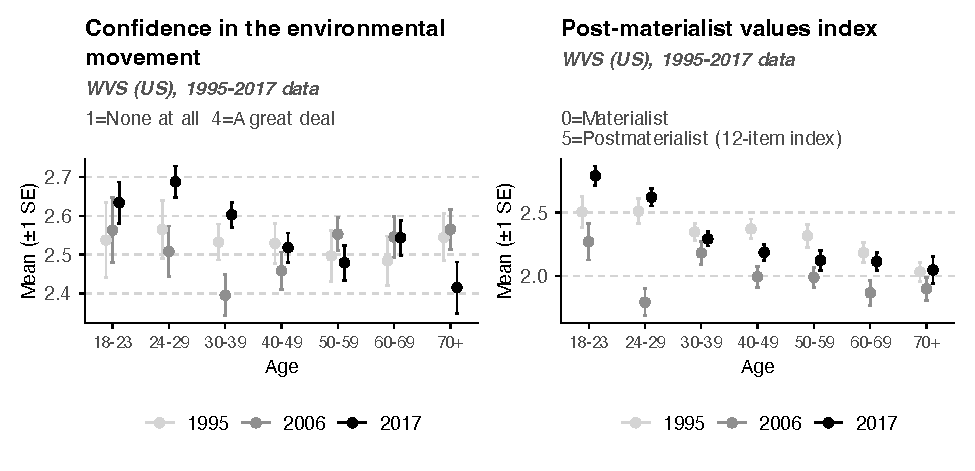
\includegraphics[width=\linewidth]{graphs/pair_postmaterial.pdf}
\end{figure}

Lastly, young Americans seem increasingly less confident in the U.S. government.

\begin{figure}[H]
    \centering
    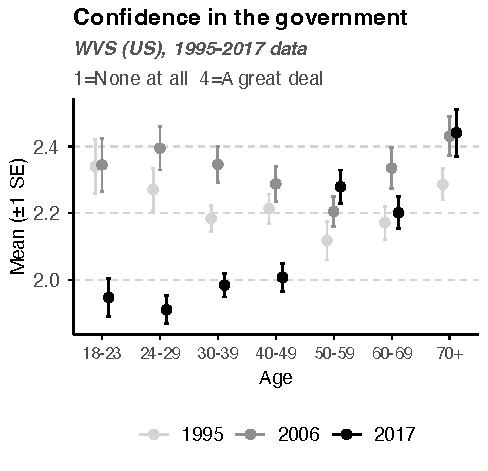
\includegraphics[width=0.5\linewidth]{graphs/WVS_E069_11_evl.pdf}
\end{figure}

\subsection{Gelbach decomposition}

Methodology: Our Gelbach decomposition compares a ``short'' model with only age as a covariate to a ``full'' model with age and many other variables (in this case, beliefs) as covariates. Our full model will feature a smaller coefficient (in absolute value) on the age covariate, suggesting an omitted variable bias in the short model that will be attributed to different belief covariates. If a belief is negatively correlated with age and positively correlated with demand for redistribution (or vice-versa), it will be an important/highly-ranked contributor in the Gelbach decomposition. If it is correlated with age but not preferences, or preferences but not age, it will not show up in the decomposition.

As we would expect, zerosumrich is highly-ranked because it is negatively correlated with age and positively correlated with preferences. However, taxdemotivates and gapmotivates are unimportant in the decomposition (i.e., do not explain the age gradient) because, while they are highly correlated with preferences, they are not correlated with age. For the progressivity outcome, beliefs about zero-sum wealth and zero-sum DEI combine to explain the majority of the age gradient.

\begin{figure}[H]
    \centering
    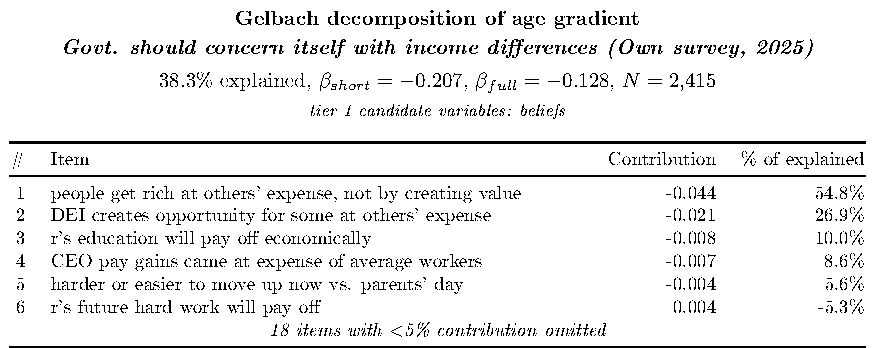
\includegraphics[width=\linewidth]{tables/05_prolific_shouldconcern_tier1.pdf}
\end{figure}
\begin{figure}[H]
    \centering
    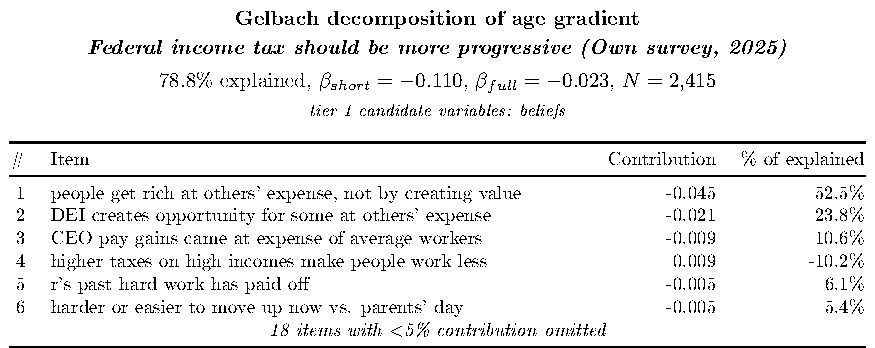
\includegraphics[width=\linewidth]{tables/07_prolific_progressivity_tier1.pdf}
\end{figure}

Cross-checking with outside surveys, data from \cite{chinoy2026zero} yields similar findings: beliefs about zero-sum wealth, race/discrimination, and opportunity combine to explain a large portion of the gradient. 

\begin{figure}[H]
    \centering
    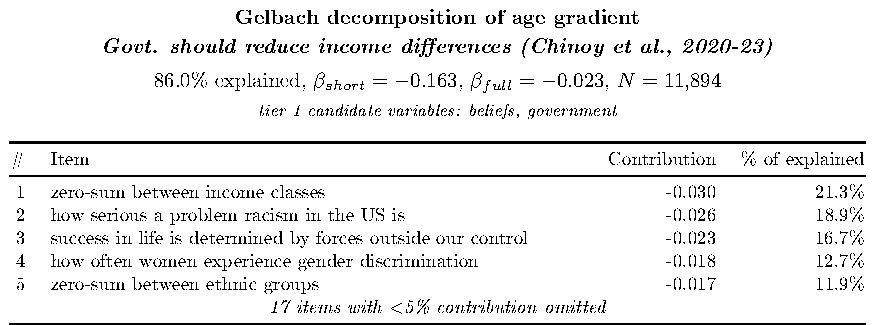
\includegraphics[width=\linewidth]{tables/01_chinoy_gov_outcome_tier1.pdf}
\end{figure}

The GSS decomposition follows similar themes, but features a slightly different set of beliefs: structural advantages of the rich and conflict between the rich and poor. 

\begin{figure}[H]
    \centering
    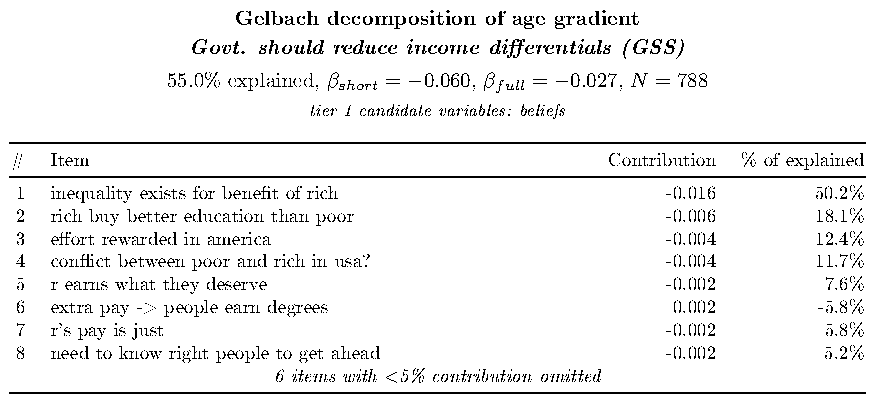
\includegraphics[width=\linewidth]{tables/03_gss_goveqinc_tier1.pdf}
\end{figure}

\newpage
\section{Why did beliefs change?}

\todo{Can look into growth during formative years, inequality, and exposure to diverse groups. Emphasize zero-sum wealth/income vs. zero-sum race/social equality, since a shock may move them in opposite directions (not explored in \cite{chinoy2026zero}).}

\section{Conclusion}

\bibliographystyle{ecta} % ecta apalike
\bibliography{refs}

\end{document}